% =====================================================================
% Stage 1 Concept and Feasibility Report -- Kenneth Dialogo
% Follows Table 1 of "Writing the Stage 1 Concept and Feasibility Report"
% (Salik). Identifiers carried from the frozen proposal: N1-N3,
% REQ-AC-01..12, R1-R3 (now risks), A1-A4, D1-D2, platform C1-C4.
%
% BEFORE PRINTING, search for "??" and replace every \Lref{...} with the
% real logbook entry number. Nothing here is invented:
% every number comes from evidence/.
% Compile in Overleaf (IEEEtran). Limit: 3-4 printed pages.
% =====================================================================
\documentclass[conference]{IEEEtran}

\usepackage{graphicx}
\usepackage{amsmath}
\usepackage{booktabs}
\usepackage{tikz}
\usetikzlibrary{positioning}

% logbook entry still to be numbered: prints L-?? with a hint
\newcommand{\Lref}[1]{L-\textbf{??}\textsuperscript{\tiny #1}}

\title{Wearable Lifestyle Activity Classifier with Wireless Reporting}

\author{
\IEEEauthorblockN{Kenneth Dialogo}
\IEEEauthorblockA{247-519-VA Project I -- Stage 1 Concept and Feasibility Report\\
Vanier College, November 18, 2026}
}

\begin{document}
\maketitle

% =====================================================================
\section{Change Log}
\label{sec:changes}

Table~\ref{tab:changes} lists every departure from the frozen
proposal. No requirement was added, removed or renumbered.

\begin{table}[h]
\centering
\footnotesize
\setlength{\tabcolsep}{3pt}
\caption{Change log. Every row names the logbook entry that explains it.}
\label{tab:changes}
\begin{tabular}{p{1.45cm}p{5.35cm}p{1.0cm}}
\toprule
\textbf{Item} & \textbf{Change and reason} & \textbf{Entry} \\
\midrule
REQ-AC-02, A2 & Training and test data: nine PAMAP2 wearers
(public dataset, hand IMU on the dominant wrist) instead of five
volunteers. Same placement as the watch; more wearers for
leave-one-wearer-out; outside data allowed by the instructor. &
\Lref{data} \\
REQ-AC-01 & Class definitions fixed: sedentary = lying, sitting,
standing, watching TV, computer work, car driving; stairs and
housework are used for testing only, not training. &
\Lref{classes} \\
Concept B & The watch shows a new label only after three agreeing
1.5\,s windows (4.5\,s), to stop the label flickering. This adds
4.5\,s before a change is reported (REQ-AC-03). &
\Lref{smooth} \\
Companion computer & A Raspberry Pi Zero 2 W runs the message
broker, the receiver and the dashboard. Reports use MQTT to my own
broker (a public broker was rejected for privacy and
repeatability); HTTP is kept as a backup. &
\Lref{mqtt} \\
REQ-AC-06 & Watch partition scheme changed from the 1.25\,MB default
to a 32\,MB scheme after the first compile used 82\,\% of program
storage. &
\Lref{C6} \\
REQ-AC-04, 05 & Test set-up: the 500\,ms / 20\,\% degradation is
applied at the Pi in both directions; the 60\,s outage is made by
stopping the broker (not by cutting the radio). &
\Lref{C4}, \Lref{C5} \\
Custom board & One thigh sensor; the chest site is dropped (the signed
form allows chest and/or thigh). Fewer parts to build this term. &
\Lref{thigh} \\
A5 (new) & Assumption added: the thigh sensor reads without I2C
errors during motion (tested by C16). &
\Lref{A5} \\
\bottomrule
\end{tabular}
\end{table}

% =====================================================================
\section{Concept Alternatives}
\label{sec:concepts}
% CHECK: keep this table only if your logbook has the criteria and
% weights dated BEFORE the scores. If not, write them in the logbook
% now, say so honestly in that entry, and then score.

Four technology-level concepts were compared; each fails for a
different reason. \textbf{A}, wrist-only learned classifier on the
wearable, fails when arm motion does not follow body motion.
\textbf{B}, wrist plus chest and/or thigh sensing fused on the
wearable, fails on link or timing problems between sites.
\textbf{C}, raw motion streamed to the computer for classification,
fails on network load, on any outage, and on the course rule that
the computer never runs the model. \textbf{D}, fixed thresholds with
no learned model, fails on wearers whose gait differs from the
thresholds and is not AI. The criteria and weights were recorded
before scoring (\Lref{criteria}), with one must-pass rule: the
concept must be able to answer the signed PoC question.

\begin{table}[h]
\centering
\footnotesize
\caption{Concept comparison (1 to 5, 5 best), $S_j=\sum_i w_i s_{ij}$.}
\label{tab:concepts}
\begin{tabular}{p{2.7cm}ccccc}
\toprule
\textbf{Criterion} & $w_i$ & \textbf{A} & \textbf{B} & \textbf{C} & \textbf{D} \\
\midrule
Requirement coverage  & 0.40 & 4 & 5 & 3 & 3 \\
Remaining uncertainty & 0.30 & 4 & 2 & 2 & 3 \\
Buildable this term   & 0.20 & 5 & 3 & 4 & 4 \\
Cost                  & 0.10 & 5 & 4 & 5 & 5 \\
\midrule
Total $S_j$           & 1.00 & 4.30 & 3.60 & 3.10 & 3.40 \\
Answers PoC question? & --   & No & Yes & No & No \\
\bottomrule
\end{tabular}
\end{table}

\textbf{Chosen: B}, the only concept that passes the must-pass rule.
A scores highest but cannot measure whether fusion helps; it is kept
as B's fallback tier (REQ-AC-10), and it is the tier the Stage 1
evidence covers. C lost because the computer would run the model and
classification stops during an outage (fails REQ-AC-05, 06). D lost
because it has no learned model (fails REQ-AC-06, 08).

\begin{figure}[h]
\centering
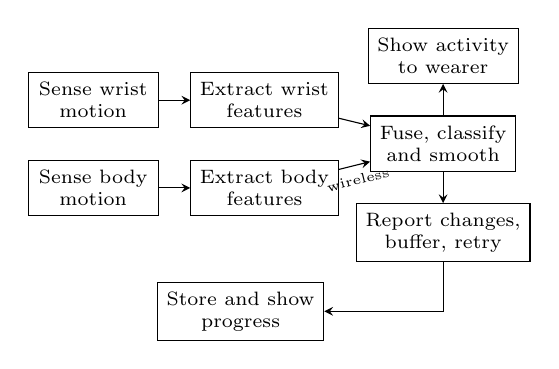
\begin{tikzpicture}[
  font=\scriptsize,
  fb/.style={draw, rectangle, minimum width=1.65cm, minimum height=0.7cm, align=center},
  >=stealth, node distance=0.4cm and 0.4cm]
\node[fb] (sw) {Sense wrist\\motion};
\node[fb, below=of sw] (sb) {Sense body\\motion};
\node[fb, right=of sw] (ew) {Extract wrist\\features};
\node[fb, right=of sb] (eb) {Extract body\\features};
\node[fb, right=0.4cm of ew, yshift=-0.55cm] (fc) {Fuse, classify\\and smooth};
\node[fb, above=of fc] (fb2) {Show activity\\to wearer};
\node[fb, below=of fc] (rp) {Report changes,\\buffer, retry};
\node[fb, left=of rp, yshift=-1.0cm] (lg) {Store and show\\progress};
\draw[->] (sw) -- (ew);
\draw[->] (sb) -- (eb);
\draw[->] (ew) -- (fc);
\draw[->] (eb) -- node[below, sloped, font=\tiny] {wireless} (fc);
\draw[->] (fc) -- (fb2);
\draw[->] (fc) -- (rp);
\draw[->] (rp) |- (lg);
\end{tikzpicture}
\caption{Chosen concept as functional blocks. If body features are
missing, classification falls back to the wrist.}
\label{fig:blocks}
\end{figure}

% =====================================================================
\section{Feasibility Case}
\label{sec:feasibility}

Table~\ref{tab:claims} gives each claim with its kind of evidence,
its logbook entry and its status. The evidence files are in the
project repository, folder \texttt{evidence}, indexed by
\texttt{claims\_register.csv}.
Pass criteria were written in the logbook before each test. A pass
fraction is $p=n_\mathrm{ok}/N$.

\begin{table*}[t]
\centering
\footnotesize
\setlength{\tabcolsep}{3pt}
\caption{Feasibility case. Every claim names the requirement it tests, its kind of evidence, its logbook entry and its status.}
\label{tab:claims}
\begin{tabular}{p{0.45cm}p{1.35cm}p{4.3cm}p{1.35cm}p{0.95cm}p{6.1cm}p{1.45cm}}
\toprule
\textbf{ID} & \textbf{Tests} & \textbf{Claim} & \textbf{Class} & \textbf{Source} & \textbf{Evidence (or planned check)} & \textbf{Status} \\
\midrule
C1 & REQ-AC-01 & The watch shows the correct label live in a scripted sit/walk/run session. & Measured & \Lref{C1} & Nov 15, 2+2+2 min: correct label 100\,\% of the time for each activity (criterion $\geq$90\,\%, first 10\,s after a change ignored); right label after 0.0/7.3/5.8\,s. & Supported \\
C2 & REQ-AC-02 & Leave-one-wearer-out mean error $\leq$15\,\%. & Measured & \Lref{C2} & 9 PAMAP2 wearers: mean 3.3\,\%, worst wearer 6.7\,\%; 1.5\,\% with the 3-window smoothing; logistic-regression baseline 3.4\,\%. Wrist only; not yet on several wearers of this watch. & Partly supported \\
C3 & REQ-AC-03 & On a healthy link every report arrives within 10\,s. & Measured & \Lref{C3} & C1 session: $p=40/40$, median 0.04\,s, max 0.14\,s, none resent or lost. 6 of the 30 minutes the method calls for. & Partly supported \\
C4 & REQ-AC-04 & With 500\,ms delay and 20\,\% loss every report arrives within 30\,s. & Measured & \Lref{C4} & Nov 16, 6 min: $p=22/24$; median 2.07\,s; a heartbeat resent 14 times (37.9\,s) held up the walking change behind it (53.1\,s). None lost. & Unsupported \\
C5 & REQ-AC-05 & After a 60\,s outage every buffered report arrives, none lost. & Measured & \Lref{C5} & Broker stopped 60\,s: nothing arrived for 65\,s; both changes made during it arrived afterwards with their real times; 0 missing sequence numbers. & Supported \\
C6 & REQ-AC-06 & The trained classifier fits in the watch's memory (C1). & Measured & \Lref{C6} & Whole sketch with model (10 trees, depth 6, 654 nodes): 1\,075\,030\,B program (3\,\% of the 32\,MB scheme; 82\,\% of the default), 72\,888\,B RAM (22\,\%). & Supported \\
C7 & REQ-AC-07 & Board feature packets reach the watch wirelessly. & -- & -- & Board not built. Planned: packet count at the watch during a live session. & Open \\
C8 & REQ-AC-08 & Firmware and pipeline deploy from one documented command. & Measured & \Lref{C8} & Nov 14: one command installed broker, receiver and dashboard on a fresh Pi (19:01--19:16). Watch upload is still manual. & Partly supported \\
C9 & REQ-AC-09 & Wrist-only, board-only and fused error reported side by side. & -- & -- & Needs board recordings; the dataset used is wrist only. & Open \\
C10 & REQ-AC-10 & With the board unplugged, reports continue with the right sensor tag. & -- & -- & Needs the board. Reports already carry the tag ``wrist''. & Open \\
C11 & REQ-AC-11 & 30-min scripted session: $\geq$85\,\% of 1-min intervals correct; active minutes reported. & -- & \Lref{C11} & Planned: plan sit 10, walk 8, run 4, sit 8 min, scored minute by minute. % UPDATE with your result
& Open \\
C12 & REQ-AC-12 & The computer shows current-session active minutes beside previous sessions. & Measured & \Lref{C12} & Nov 15 dashboard: 4.0 active min, ``+4.0 min compared with last session'', chart of the last 10 sessions. & Supported \\
C13 & A1 & In one room the watch reaches the board and the computer. & Measured & \Lref{C3} & Watch to Pi in one room: 0 lost in C1, C5 tests. Board part not built. & Partly supported \\
C14 & A3 & Motion features separate sedentary, walking and running. & Measured & \Lref{C14} & Own watch, 121 windows: 8 of 10 features separate all three (middle 80\,\% do not overlap); cadence does not. Agrees with PAMAP2. & Supported \\
C15 & A4 & The watch's figures (C1--C4) match its datasheet. & Assumed & -- & Taken from the vendor wiki; settled by checking the datasheet. & Open \\
C16 & A5 & The thigh sensor reads without I2C errors while walking and running. & -- & -- & Needs the board. Planned: error count over a session. & Open \\
\bottomrule
\end{tabular}
\end{table*}

\textbf{Classification (C1, C2, C14).} The model is a random forest
of 10 trees trained on ten orientation-free features from 1.5\,s
windows at 40\,Hz, and it runs on the watch. On the dataset it is
far inside the 15\,\% target, and in the live test it gave the right
label for the whole of each activity. Live switching takes 6--7\,s,
which is the 4.5\,s smoothing plus window timing. C2 stays partly
supported because the error comes from a public dataset with a
different sensor, and three of the nine wearers have no running
data.

\textbf{Link (C3--C5).} On a healthy link the delay is far below
10\,s and nothing was lost after a 60\,s outage. Under 500\,ms delay
and 20\,\% loss in both directions nothing was lost either, but
$p=22/24=0.92$ falls short of the 100\,\% the requirement asks for.
The cause is that the watch sends reports strictly in order, so one
report stuck in retries holds up the next. C4 is reported
unsupported, not adjusted.

\textbf{Board (C7, C9, C10, C16).} The thigh board is not built, so
the fusion half of the PoC question is not answered yet.

% =====================================================================
\section{Baselined Requirements}
\label{sec:baseline}

\begin{table}[h]
\centering
\footnotesize
\setlength{\tabcolsep}{3pt}
\caption{Baselined requirements, one status each.}
\label{tab:baseline}
\begin{tabular}{p{1.45cm}p{0.55cm}p{3.95cm}p{1.35cm}}
\toprule
\textbf{ID} & \textbf{Claim} & \textbf{Now (reason if changed)} & \textbf{Status} \\
\midrule
REQ-AC-01 & C1 & Kept; classes defined (Table~\ref{tab:changes}) & Supported \\
REQ-AC-02 & C2 & Kept at 15\,\%; tested on 9 PAMAP2 wearers & Partly supp. \\
REQ-AC-03 & C3 & Kept at 10\,s; full 30-min session pending & Partly supp. \\
REQ-AC-04 & C4 & Kept at 30\,s; reported unsupported, design fix planned & Unsupported \\
REQ-AC-05 & C5 & Kept; Wi-Fi outage still to repeat & Supported \\
REQ-AC-06 & C6 & Kept & Supported \\
REQ-AC-07 & C7 & Kept & Open \\
REQ-AC-08 & C8 & Kept; watch upload to be added & Partly supp. \\
REQ-AC-09 & C9 & Kept & Open \\
REQ-AC-10 & C10 & Kept & Open \\
REQ-AC-11 & C11 & Kept at 85\,\% & Open \\
REQ-AC-12 & C12 & Kept & Supported \\
\bottomrule
\end{tabular}
\end{table}

% =====================================================================
\section{Risk Register}
\label{sec:risks}

The proposal's uncertainties R1--R3 are now risks with estimated
probabilities; R4--R7 were uncovered by the work. Probability $p$ and
consequence $c$ run from 1 to 4, $P=p\times c$, and ties go to the
higher consequence (Table~\ref{tab:risks}, Fig.~\ref{fig:matrix}).

\begin{table}[h]
\centering
\footnotesize
\setlength{\tabcolsep}{3pt}
\caption{Risks ranked by $P=p\times c$.}
\label{tab:risks}
\begin{tabular}{p{0.45cm}p{4.6cm}cccc}
\toprule
\textbf{ID} & \textbf{Risk (evidence behind $p$)} & $p$ & $c$ & $P$ & \textbf{Rank} \\
\midrule
R4 & Board not built in time; C7, C9, C10, C16 stay open & 3 & 3 & 9 & 1 \\
R2 & Reports late on a degraded link (C4: 2 of 24 late) & 4 & 2 & 8 & 2 \\
R1 & Model does not hold for other wearers of this watch (one wearer tested so far) & 2 & 3 & 6 & 3 \\
R3 & Fusion does not beat wrist-only (wrist already 3.3\,\%) & 3 & 2 & 6 & 4 \\
R6 & Watch cannot reach the Pi after a restart (seen Nov 14) & 3 & 2 & 6 & 5 \\
R5 & Pi Zero overloaded or SD card damaged (browser froze it) & 2 & 2 & 4 & 6 \\
R7 & Program storage runs out (closed: C6, now 3\,\%) & 1 & 3 & 3 & 7 \\
\bottomrule
\end{tabular}
\end{table}

\begin{figure}[h]
\centering
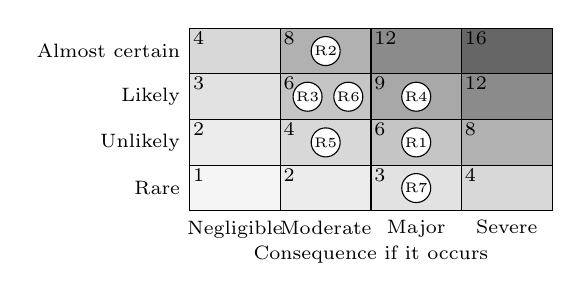
\begin{tikzpicture}[x=1.15cm, y=0.58cm, font=\scriptsize]
\foreach \p in {1,...,4} {
  \foreach \c in {1,...,4} {
    \pgfmathtruncatemacro{\P}{\p*\c}
    \pgfmathsetmacro{\shade}{min(60,\P*3.8)}
    \fill[black!\shade] (\c-1,\p-1) rectangle (\c,\p);
    \draw (\c-1,\p-1) rectangle (\c,\p);
    \node[anchor=north west, inner sep=1pt] at (\c-1,\p) {\P};
  }
}
\foreach \l [count=\i] in {Rare,Unlikely,Likely,Almost certain}
  \node[anchor=east] at (0,\i-0.5) {\l};
\foreach \l [count=\i] in {Negligible,Moderate,Major,Severe}
  \node[anchor=north] at (\i-0.5,0) {\l};
\node at (2,-0.95) {Consequence if it occurs};
\tikzset{r/.style={draw, circle, fill=white, inner sep=0.6pt, font=\tiny}}
\node[r] at (2.5,2.5) {R4};
\node[r] at (1.5,3.5) {R2};
\node[r] at (2.5,1.5) {R1};
\node[r] at (1.3,2.5) {R3};
\node[r] at (1.75,2.5) {R6};
\node[r] at (1.5,1.5) {R5};
\node[r] at (2.5,0.5) {R7};
\end{tikzpicture}
\caption{Risk matrix; darker cells need attention first.}
\label{fig:matrix}
\end{figure}

\begin{table}[h]
\centering
\footnotesize
\caption{Top-ranked risk, R4, in six fields.}
\label{tab:toprisk}
\begin{tabular}{p{1.6cm}p{5.8cm}}
\toprule
\textbf{Field} & \textbf{Entry} \\
\midrule
Statement & The chest/thigh board is not built and tested in time. \\
Assumption & The ESP32 board and MPU-6050 module can be wired, programmed and linked to the watch within two weeks. \\
Consequence & C7, C9, C10, C16 stay open; the fusion half of the PoC question is unanswered; wrist-only becomes the primary design (R3 mitigation). \\
Probability & Likely (3): no board work logged yet; all Stage 1 time went to the wrist tier and the link. \\
Evidence required & Board packets counted at the watch (C7), then wrist/board/fused error on the same folds (C9). \\
Mitigation & Build the thigh board first (one sensor), reuse the watch's existing reporting code, and record own data with it. \\
\bottomrule
\end{tabular}
\end{table}

% =====================================================================
\section{Gate 1 Readiness}
\label{sec:readiness}

The wrist tier of the concept works on the watch: the model fits
with room to spare (C6), gives the right label live (C1), and its
features separate the three activities on my own wrist (C14), with
a leave-one-wearer-out error of 3.3\,\% on the dataset (C2). The link
meets its healthy-link and outage targets (C3, C5), and the dashboard
compares sessions (C12). Two shortfalls are reported as they are: on
a degraded link 2 of 24 reports were late (C4, unsupported), and the
whole board half is open (C7, C9, C10, C16), so the fusion question
in the PoC is not answered. I expect \textbf{proceed with
conditions}: (1) build the thigh board and run C7 and C9 by
\textbf{[date]}; (2) send activity changes ahead of heartbeats and
retest C4 by \textbf{[date]}; (3) complete the 30-minute session
(C11) by \textbf{[date]}.

\vspace{2pt}
\noindent{\footnotesize\emph{AI use:} an AI assistant helped draft
wording, the analysis and test scripts, and the firmware link code;
every number above was measured by me and is recorded in the cited
logbook entry.}

\end{document}
